\documentclass[12pt]{report}
\usepackage[utf8]{inputenc}
\usepackage[russian]{babel}
%\usepackage[14pt]{extsizes}
\usepackage{listings}
\usepackage{graphicx}
\usepackage{amsmath,amsfonts,amssymb,amsthm,mathtools} 
\usepackage{pgfplots}
\usepackage{filecontents}
\usetikzlibrary{datavisualization}
\usetikzlibrary{datavisualization.formats.functions}

% Для листинга кода:
\lstset{ %
language=haskell,                 % выбор языка для подсветки (здесь это С)
basicstyle=\small\sffamily, % размер и начертание шрифта для подсветки кода
numbers=left,               % где поставить нумерацию строк (слева\справа)
numberstyle=\tiny,           % размер шрифта для номеров строк
stepnumber=1,                   % размер шага между двумя номерами строк
numbersep=5pt,                % как далеко отстоят номера строк от подсвечиваемого кода
showspaces=false,            % показывать или нет пробелы специальными отступами
showstringspaces=false,      % показывать или нет пробелы в строках
showtabs=false,             % показывать или нет табуляцию в строках
frame=single,              % рисовать рамку вокруг кода
tabsize=2,                 % размер табуляции по умолчанию равен 2 пробелам
captionpos=t,              % позиция заголовка вверху [t] или внизу [b] 
breaklines=true,           % автоматически переносить строки (да\нет)
breakatwhitespace=false, % переносить строки только если есть пробел
escapeinside={\#*}{*)}   % если нужно добавить комментарии в коде
}

\usepackage[left=2cm,right=2cm, top=2cm,bottom=2cm,bindingoffset=0cm]{geometry}
% Для измененных титулов глав:
\usepackage{titlesec, blindtext, color} % подключаем нужные пакеты
\definecolor{gray75}{gray}{0.75} % определяем цвет
\newcommand{\hsp}{\hspace{20pt}} % длина линии в 20pt
% titleformat определяет стиль
\titleformat{\chapter}[hang]{\Huge\bfseries}{\thechapter\hsp\textcolor{gray75}{|}\hsp}{0pt}{\Huge\bfseries}


% plot
\usepackage{pgfplots}
\usepackage{filecontents}
\usetikzlibrary{datavisualization}
\usetikzlibrary{datavisualization.formats.functions}

\begin{document}
%\def\chaptername{} % убирает "Глава"
\thispagestyle{empty}
\begin{titlepage}
	\noindent \begin{minipage}{0.15\textwidth}
	
\includegraphics[width=\linewidth]{b_logo}
	\end{minipage}
	\noindent\begin{minipage}{0.9\textwidth}\centering
		\textbf{Министерство науки и высшего образования Российской Федерации}\\
		\textbf{Федеральное государственное бюджетное образовательное учреждение высшего образования}\\
		\textbf{~~~«Московский государственный технический университет имени Н.Э.~Баумана}\\
		\textbf{(национальный исследовательский университет)»}\\
		\textbf{(МГТУ им. Н.Э.~Баумана)}
	\end{minipage}
	
	\noindent\rule{18cm}{3pt}
	\newline\newline
	\noindent ФАКУЛЬТЕТ $\underline{\text{«Информатика и системы управления»}}$ \newline\newline
	\noindent КАФЕДРА $\underline{\text{«Программное обеспечение ЭВМ и информационные технологии»}}$\newline\newline\newline\newline\newline
	
	
	\begin{center}
		\noindent\begin{minipage}{1.3\textwidth}\centering
			\Large\textbf{  Лабораторная работа № 1}\newline
			\textbf{по дисциплине "Анализ алгоритмов"}\newline\newline
		\end{minipage}
	\end{center}
	
	\noindent\textbf{Тема} $\underline{\text{Расстояние Левенштейна}}$\newline\newline
	\noindent\textbf{Студент} $\underline{\text{Романов А.В.}}$\newline\newline
	\noindent\textbf{Группа} $\underline{\text{ИУ7-53Б}}$\newline\newline
	\noindent\textbf{Оценка (баллы)} $\underline{\text{~~~~~~~~~~~~~~~~~~~~~~~~~~~}}$\newline\newline
	\noindent\textbf{Преподаватели} $\underline{\text{Волкова Л.Л., Строганов Ю.В.}}$\newline\newline\newline
	
	\begin{center}
		\vfill
		Москва~---~\the\year
		~г.
	\end{center}
\end{titlepage}


\tableofcontents

\newpage
\chapter*{Введение}
\addcontentsline{toc}{chapter}{Введение}
\textbf{Расстояние Левенштейна} - минимальное количество операций вставки одного символа, удаления одного символа и замены одного символа на другой, необходимых для превращения одной строки в другую.
\newline

Расстояние Левенштейна применяется в теории информации и компьютерной лингвистике для:

\begin{itemize}
	\item исправления ошибок в слове
	\item сравнения текстовых файлов утилитой diff
	\item в биоинформатике для сравнения генов, хромосом и белков
\end{itemize}

Целью данной лабораторной работы: 
\begin{enumerate}
	\item Изучение метода динамического программирования на материале алгоритмов Левенштейна и Дамерау-Левенштейна.
	\item Оценка реализаций алгоритмов Левенштейна и Дамерау-Левенштейна.
\end{enumerate}

Задачи данной лабораторной работы:
\begin{enumerate}
  	\item Изучение алгоритмов Левенштейна и Дамерау-Левенштейна;
	\item Применение метода динамического программирования для матричной реализации указанных алгоритмов; 
	\item Получение практических навыков реализации указанных алгоритмов: матричные и рекурсивные версии; 
	\item Сравнительный анализ линейной и рекурсивной реализаций выбранного алгоритма определения расстояния между строками по затрачиваемым ресурсам (времени и памяти); 
	\item Экспериментальное подтверждение различий во временнóй эффективности рекурсивной и
нерекурсивной реализаций выбранного алгоритма; 
	\item Описание и обоснование полученных результатов в отчете о выполненной лабораторной
работе, выполненного как расчётно-пояснительная записка к работе. 
\end{enumerate}


\chapter{Аналитическая часть}

Расстояние Левенштейна \cite{Levenshtein} между двумя строками — это минимальное количество операций вставки, удаления и замены, необходимых для превращения одной строки в другую.


Цены операций могут зависеть от вида операции (вставка (insert), удаление (delete), замена (replace) и/или от участвующих в ней символов, отражая разную вероятность разных ошибок при вводе текста, и т. п. В общем случае:

\begin{itemize}

	\item $w(a,b)$ — цена замены символа $a$ на символ $b$.

	\item $w(\lambda,b)$ — цена вставки символа $b$.

	\item $w(a,\lambda)$ — цена удаления символа $a$.

\end{itemize} 


Для решения задачи о редакционном расстоянии необходимо найти последовательность замен, минимизирующую суммарную цену. Расстояние Левенштейна является частным случаем этой задачи при

\begin{itemize}

	\item $w(a,a)=0$.

	\item $w(a,b)=1, \medspace a \neq b$.

	\item $w(\lambda,b)=1$.

	\item $w(a,\lambda)=1$.

\end{itemize} 


\section{Рекурсивный алгоритм нахождения расстояния Левенштейна}

Расстояние Левенштейна между двумя строками a и b может быть вычислено по формуле \ref{eq:D}, где $|a|$ означает длину строки $a$; $a[i]$ — i-ый символ строки $a$ , функция $D(i, j)$ определена как:
\begin{equation}
\label{eq:D}
D(i, j) = \begin{cases}
0 &\text{i = 0, j = 0}\\
i &\text{j = 0, i > 0}\\
j &\text{i = 0, j > 0}\\
\min \lbrace \\
\qquad D(i, j-1) + 1\\
\qquad D(i-1, j) + 1 &\text{i > 0, j > 0}\\
\qquad D(i-1, j-1) + m(a[i], b[j]) &\text(\ref{eq:m})\\
\rbrace
\end{cases},
\end{equation}

а функция \ref{eq:m} определена как:
\begin{equation}
\label{eq:m}
m(a, b) = \begin{cases}
0, &\text{если a = b,}\\
1 &\text{иначе}
\end{cases}.
\end{equation}

Рекурсивный алгоритм реализует формулу \ref{eq:D}.
Функция $D$ составлена из следующих соображений:
\begin{enumerate}
	\item Для перевода из пустой строки в пустую требуется ноль операций;
	\item Для перевода из пустой строки в строку $a$ требуется $|a|$ операций;
	\item Для перевода из строки $a$ в пустую требуется $|a|$ операций;
	\item Для перевода из строки $a$ в строку $b$ требуется выполнить последовательно некоторое количество операций (удаление, вставка, замена) в некоторой последовательности. Последовательность проведения любых двух операций можно поменять, порядок проведения операций не имеет никакого значения. Полагая, что $a', b'$  — строки $a$ и $b$ без последнего символа соответственно, цена преобразования из строки $a$ в строку $b$ может быть выражена как:
	\begin{enumerate}
		\item Сумма цены преобразования строки $a$ в $b$ и цены проведения операции удаления, которая необходима для преобразования $a'$ в $a$;
		\item Сумма цены преобразования строки $a$ в $b$  и цены проведения операции вставки, которая необходима для преобразования $b'$ в $b$;
		\item Сумма цены преобразования из $a'$ в $b'$ и операции замены, предполагая, что $a$ и $b$ оканчиваются разные символы;
		\item Цена преобразования из $a'$ в $b'$, предполагая, что $a$ и $b$ оканчиваются на один и тот же символ.
	\end{enumerate}
	Минимальной ценой преобразования будет минимальное
	значение приведенных вариантов.
\end{enumerate}

\section{Матричный алгоритм нахождения расстояния Левенштейна}

Прямая реализация формулы \ref{eq:D} может быть малоэффективна по времени исполнения при больших $i, j$, т. к. множество промежуточных значений $D(i, j)$ вычисляются заново множество раз подряд. Для оптимизации нахождения расстояния Левенштейна можно использовать матрицу в целях хранения соответствующих промежуточных значений. В таком случае алгоритм представляет собой построчное заполнение матрицы

$A_{|a|,|b|}$ значениями $D(i, j)$.


\section{Рекурсивный алгоритм нахождения расстояния Левенштейна с заполнением матрицы}

\label{sec:recmat}


Рекурсивный алгоритм заполнения можно оптимизировать по времени выполнения с использованием матричного алгоритма. Суть данного метода заключается в параллельном заполнении матрицы при выполнении рекурсии. В случае, если рекурсивный алгоритм выполняет прогон для данных, которые еще не были обработаны, результат нахождения расстояния заносится в матрицу. В случае, если обработанные ранее данные встречаются снова, для них расстояние не находится и алгоритм переходит к следующему шагу.


\section{Расстояния Дамерау — Левенштейна}

Расстояние Дамерау — Левенштейна может быть найдено по формуле \ref{eq:d}, которая задана как
\begin{equation}
\label{eq:d}
d_{a,b}(i, j) = \begin{cases}
\max(i, j) &\text{если }\min(i, j) = 0,\\
\min \lbrace \\
\qquad d_{a,b}(i, j-1) + 1\\
\qquad d_{a,b}(i-1, j) + 1 &\text{иначе}\\
\qquad d_{a,b}(i-1, j-1) + m(a[i], b[j])\\
\qquad d_{a,b}(i-2, j-2) + 1 &\text{если }i,j > 1;\\
\qquad &\text{}a[i] = b[j-1]; \\
\qquad &\text{}b[j] = a[i-1]\\
\rbrace
\end{cases},
\end{equation}

Формула выводится по тем же соображениям, что и формула (\ref{eq:D}).
Как и в случае с рекурсивным методом, прямое применение этой формулы неэффективно по времени исполнения, то аналогично методу из \ref{sec:recmat} производится добавление матрицы для хранения промежуточных значений рекурсивной формулы.

\section{Вывод}
	В данном разделе были рассмотрены алгоритмы нахождения расстояния Левенштейна и Дамерау-Левенштейна, который является модификаций первого, учитывающего возможность перестановки соседних символов. Формулы Левенштейна и Дамерау — Левенштейна для рассчета расстояния между строками задаются рекурсивно, а следовательно, алгоритмы могут быть реализованы рекурсивно или итерационно.
	
\clearpage

\chapter{Конструкторская часть}

\section{Схемы алгоритмов}
В данной части будут рассмотрены схемы алгоритмов.

\begin{figure}[h]
	\centering
	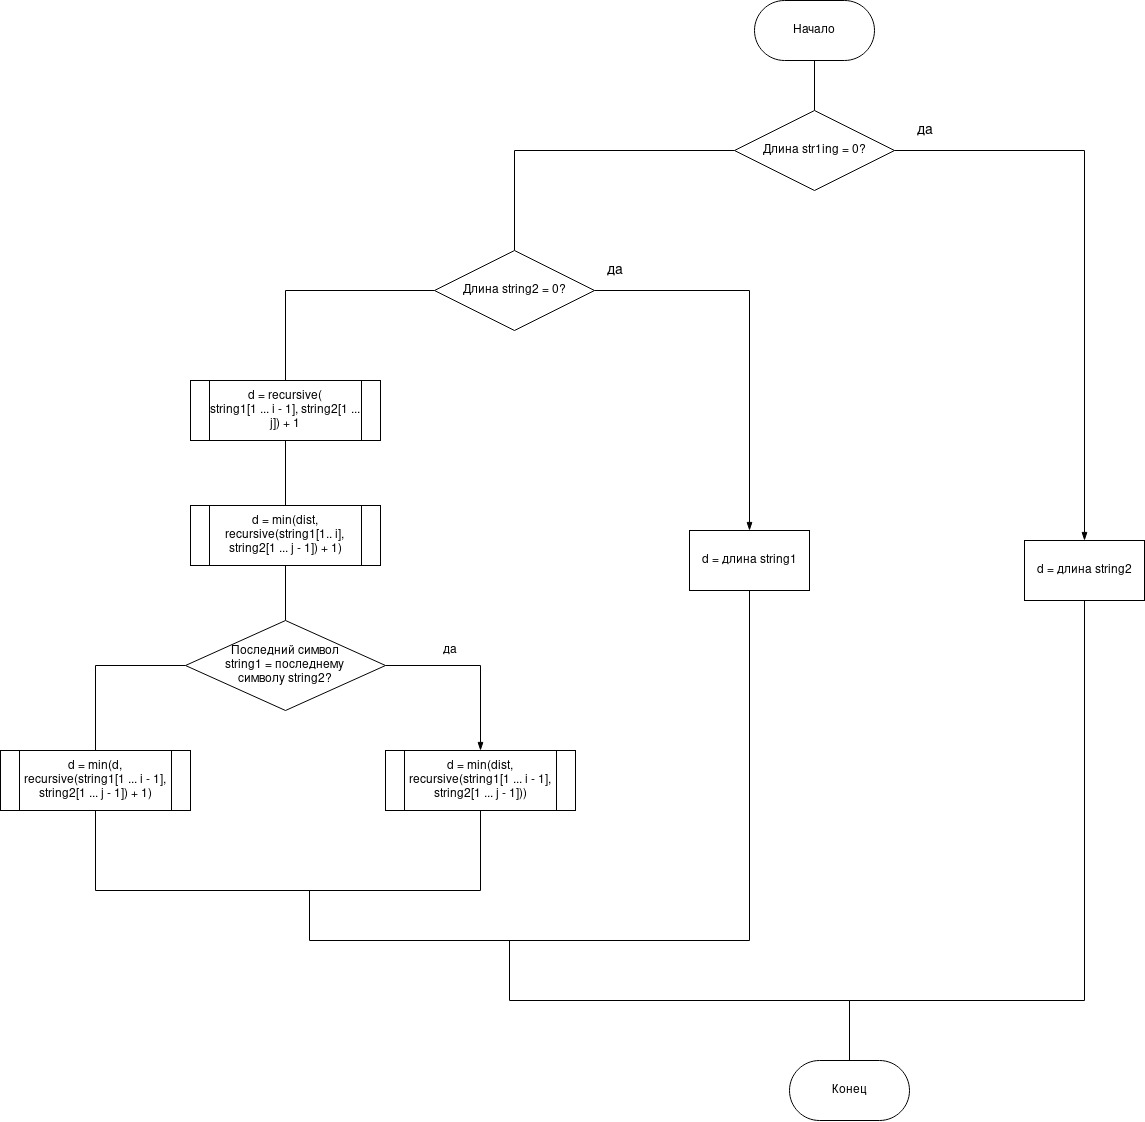
\includegraphics[width=0.75\linewidth]{rec.jpg}
	\caption{Схема рекурсивного алгоритма нахождения расстояния Левенштейна}
	\label{fig:mpr}
\end{figure}


\begin{figure}[h]
	\centering
	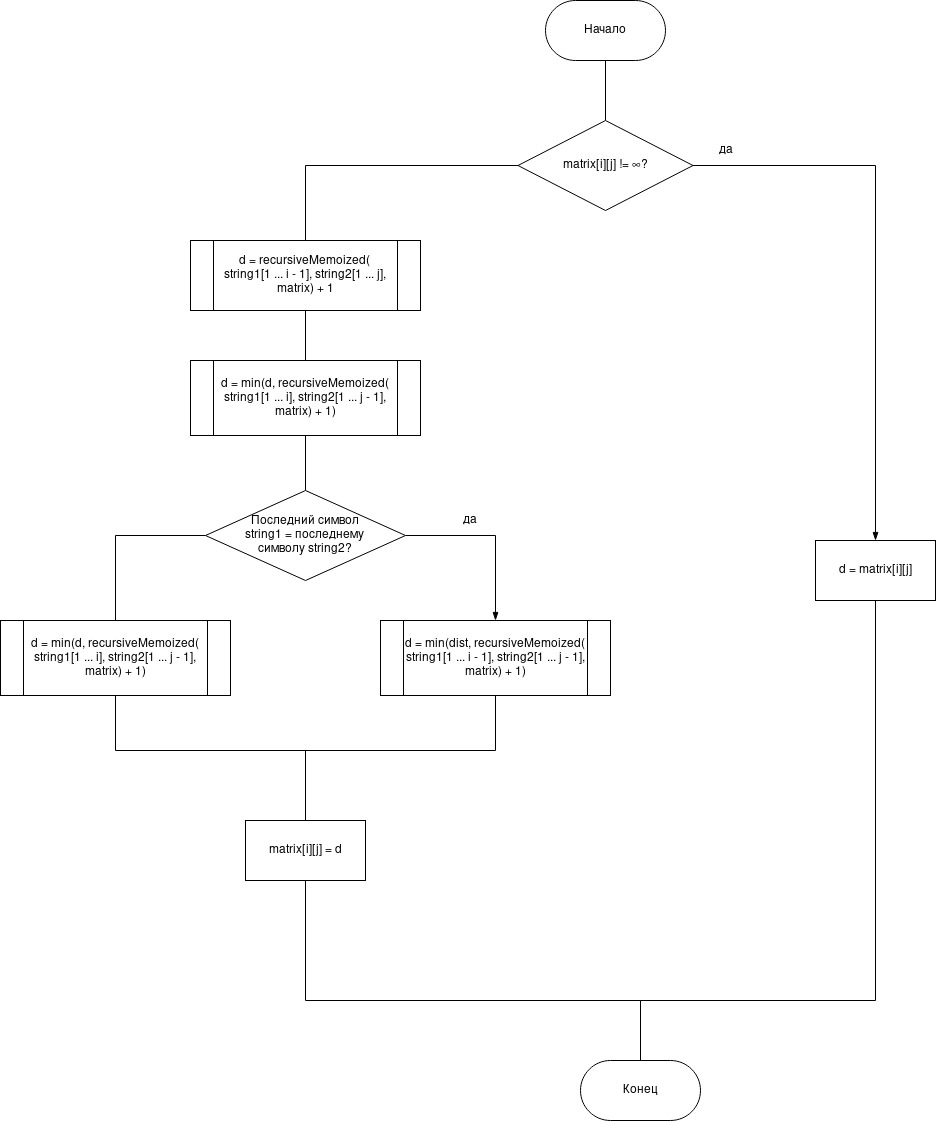
\includegraphics[scale=0.45]{mem.jpg}
	\caption{Схема рекурсивного алгоритма с мемоизацией нахождения расстояния Левенштейна}
	\label{fig:mpr}
\end{figure}


\begin{figure}[h]
	\centering
	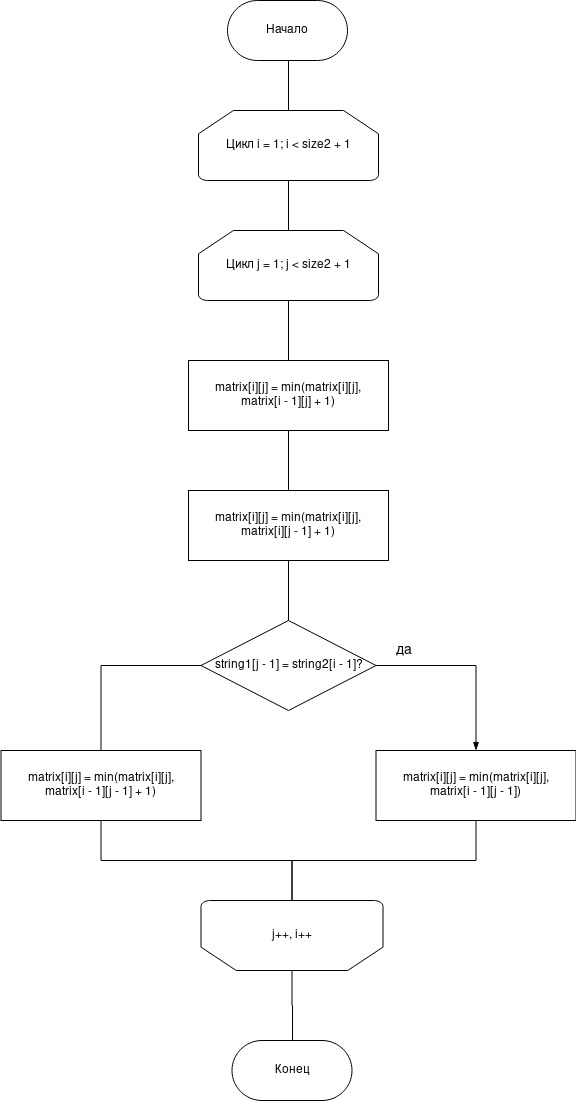
\includegraphics[scale=0.6]{iter.jpg}
	\caption{Схема итеративного алгоритма нахождения расстояния Левенштейна}
	\label{fig:mpr}
\end{figure}

\begin{figure}[h]
	\centering
	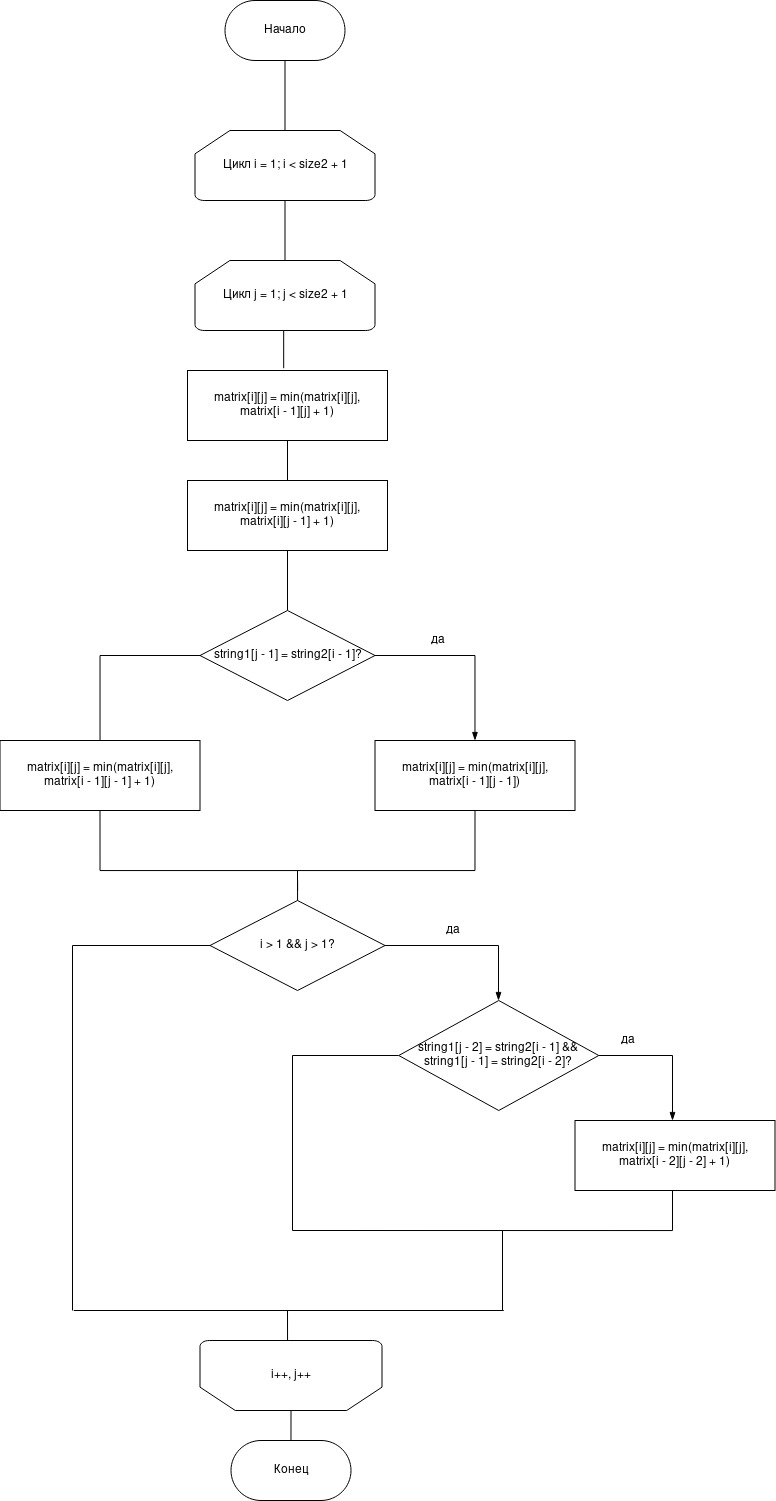
\includegraphics[scale=0.4]{iter_dl.jpg}
	\caption{Схема итеративного алгоритма нахождения расстояния Дамерау-Левенштейна}
	\label{fig:mpr}
\end{figure}

\section{Вывод}
	На основе теоретических данных, полученные в аналитическом разделе были построены схемы иследуеммых  алгоритмов.

\chapter{Технологическая часть}

\section{Требование к ПО}
\textbf{Требования к вводу:}
\begin{enumerate}
	\item На вход подаются две строки в любой раскладке (в том числе и пустые);
	\item ПО должно выводить полученное расстояние и вспомогательны матрицы;
	\item ПО должно выводить потраченную память и время;
\end{enumerate}

\section{Средства реализации}
Для реализации программы нахождения расстояние Левенштейна я выбрал язык программирования Haskell \cite{Haskell}. Данный
выбор обусловлен моим желанием расширить свои знания в области
применения данного язкыа программирования.

\section{Реализация алгоритмов}

\begin{lstlisting}[label=some-code,caption=Функция нахождения расстояния Левенштейна рекурсивно,language=Haskell]
levenshteinRecursion :: String -> String -> (Distance, Depth)
levenshteinRecursion s1 s2 = _recursion s1 s2 0
	where _recursion s1 "" n = (length s1, n)
		_recursion "" s2 n = (length s2, n)
		_recursion s1 s2 n = (score, depth) where
		(insert, curr1) = _recursion (init s1) s2 (n + 1)
		(delete, curr2) = _recursion s1 (init s2) (n + 1)
		(replace, curr3) = _recursion (init s1) (init s2) (n + 1)

		match = if last s1 == last s2 then 0 else 1
		score = min3 (insert + 1) (delete + 1) (replace + match)
		depth = max3 curr1 curr2 curr3
\end{lstlisting}

\begin{lstlisting}[label=some-code,caption=Функция нахождения расстояние Левенштейна рекурсивно с мемоизацией,language=Haskell]
levenshteinMemoized :: String -> String -> (Distance, Depth)
levenshteinMemoized s1 s2 = _memoized s1 s2 matrix 0
	where matrix = fromList (length s1 + 1) (length s2 + 1) $ repeat (-1) 
		_memoized s1 "" _ n = (length s1, n)
		_memoized "" s2 _ n = (length s2, n)
		_memoized s1 s2 mtr n = (score, depth) where
		score = min3 (insert + 1) (delete + 1) (replace + match)
		memoized = (getElem (length s1) (length s2) mtr, n + 1)
		new_mtr = setElem score (length s1, length s2) mtr 

		(insert, curr1) = if fst memoized == -1 then _memoized (init s1) s2 new_mtr (n + 1)
			else memoized
		(delete, curr2) = if fst memoized == -1 then _memoized s1 (init s2) new_mtr (n + 1)
			else memoized
		(replace, curr3) = if fst memoized == -1 then _memoized (init s1) (init s2) new_mtr (n + 1)
			else memoized

		match = if last s1 == last s2 then 0 else 1
		depth = max3 curr1 curr2 curr3
\end{lstlisting}

\begin{lstlisting}[label=some-code,caption=Функция нахождения расстояния Левенштейна итеративно,language=Haskell]
levenshteinIterative :: String -> String -> Matrix Int
levenshteinIterative s1 s2 = fromLists $ reverse $ foldl
	(\mtr i -> if head mtr == [] then [[0..length s1]] else calcRow mtr i : mtr) [[]] [0..length s2]
	where calcRow mtr i = foldl (\row j ->
			row ++ if length row == 0 then [length mtr] else [
				min3 (last row + 1) (head mtr !! j + 1) $ head mtr !! (j - 1) +
					if s1 !! (j - 1) == s2 !! (i - 1) then 0 else 1]
			) [] [0..length s1]
\end{lstlisting}


\begin{lstlisting}[label=some-code,caption=Функция нахождения расстояния Дамерау-Левенштейна матрично,language=Haskell]
damerauLevenshtein :: String -> String -> Matrix Int
damerauLevenshtein s1 s2 = fromLists $ reverse $ foldl
	(\mtr i -> if head mtr == [] then [[0..length s1]] else calcRow mtr i : mtr) [[]] [0..length s2]
	where cell mtr row i j = min3 (last row + 1) (head mtr !! j + 1) $ head mtr !! (j - 1) +
			if s1 !! (j - 1) == s2 !! (i - 1) then 0 else 1
			transposition i j = i > 1 && j > 1 && s1 !! (j - 1) == s2 !! (i - 2) && s1 !! (j - 2) == s2 !! (i - 1)
			calcRow mtr i = foldl (\row j -> row ++ [
				if length row == 0 then length mtr
				else if transposition i j then min (cell mtr row i j) (((head $ tail mtr) !! i - 2) + 1)
				else cell mtr row i j]
			) [] [0..length s1]
\end{lstlisting}

\section{Вывод}
В данном разделе были разработан исходный код четырех алгоритмов: вычисления расстояния Левенштейна рекурсивно, с заполнением матрицы
и рекурсивно с заполнением матрицы, а также вычисления расстояния
Дамерау — Левенштейна с заполнением матрицы

\chapter{Исследовательская часть}

\section{Пример работы}

Демонстрация работы программы приведена на рисунке 4.1.

\begin{figure}[h]
	\begin{center}
	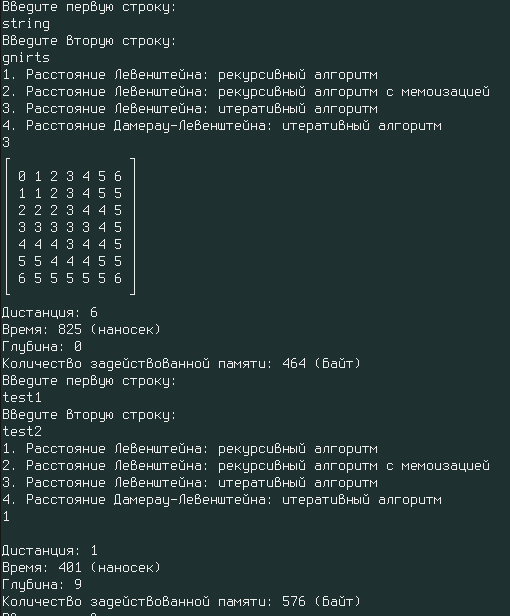
\includegraphics[scale=0.7]{primer.png}
	 \caption{Работа алгоритмов Левенштейна и Дамерау -- Левенштейна.}
	\end{center}
\end{figure}

\section{Тестовые данные}

В таблице 4.1 приведены тестовые данные, на которых было протестированно ПО.

\begin{table}[h]
	\begin{center}
		\begin{tabular}{|c c c c c|} 
			\hline
			№ & Первое слово & Второе слово & Ожидаемый результат & Полученный результат \\ [0.8ex] 
			\hline
			1 &  &  & 0 0 0 0 & 0 0 0 0\\
			\hline
			2 & kot & skat & 2 2 2 2 & 2 2 2 2\\
			\hline
			3 & kate & ktae & 2 2 1 1 & 2 2 1 1\\
			\hline
			4 & abacaba & aabcaab & 4 4 2 2 & 4 4 2 2\\
			\hline
			5 & sobaka & sboku & 3 3 3 3 & 3 3 3 3\\
			\hline
			6 & qwerty & queue & 4 4 4 4 & 4 4 4 4\\
			\hline
			7 & apple & aplpe & 2 2 1 1  & 2 2 1 1\\
			\hline
			8 &  & cat & 3 3 3 3 & 3 3 3 3\\
			\hline
			9 & parallels &  & 9 9 9 9 & 9 9 9 9\\
			\hline
			10 & bmstu & utsmb & 4 4 4 4 & 4 4 4 4\\
			\hline
		\end{tabular}
		\caption{Таблица тестовых данных}
	\end{center}
\end{table}


\section{Время выполнения алгоритмов}

В таблице 4.2. представленны замеры времени работы для каждого из алгоритмов.
\begin{table} [h!]
	\begin{center}
		\begin{tabular}{|c c c c c|} 
		 	\hline
			Длина строк & LR & LMR & LI & DLI \\  
		 	\hline
		 	10 & 30500400 & 1300 & 650 & 680\\
		 	\hline
		 	20 & NaN & 5100 & 2300 & 2500 \\
		 	\hline
			30 & NaN & 11000 & 4800 & 5200 \\
			\hline
			50 & NaN & 30000 & 12500 & 13500 \\
			\hline
			100 & NaN & 115000 & 48000 & 55000\\
			\hline
			200 & NaN & 530000 & 249000 & 528000 \\
			\hline
		\end{tabular}
	\end{center}
	\caption{Таблица времени выполнения алгоритмов (в наносекундах)}
\end{table}

\section{Оценка памяти}

\begin{filecontents}{iter.dat}
10      634
20      2367
30      4813
50      12518
100     48111
200     249057
\end{filecontents}

\begin{filecontents}{iterDl.dat}
10      681
20      2562
30      5207
50      13533
100     54078
200     527797
\end{filecontents}

\begin{filecontents}{rec.dat}
5       6771
10      32766430
\end{filecontents}

\begin{filecontents}{recWithMem.dat}
10      1313
20      5157
30      11342
50      30066
100     116134
200     529335
\end{filecontents}

\begin{tikzpicture}

\begin{axis}[
    axis lines = left,
    xlabel={len (symbols)},
    ylabel={time (ticks)},
    xmin=5, xmax=200,
    ymin=1, ymax=600000,
    legend pos=north west,
    ymajorgrids=true
]

\addplot[color=red] table[x index=0, y index=1] {iter.dat}; 
\addplot[color=orange] table[x index=0, y index=1] {iterdl.dat};
\addplot[color=blue, mark=square] table[x index=0, y index=1] {rec.dat};
\addplot[color=green, mark=square] table[x index=0, y index=1] {recwithmem.dat};

\section{Вывод}

Рекурсивный алгоритм Левенштейна работает на порядок дольше итеративных реализаций, время его работы увеличивается в геометрической прогрессии. Кроме того, рекурсивный алгоритм с мемоизацией проигрывает по памяти: так как в языке Haskell каждый объект является неизменяемым, каждый рекурсивный вызов создается новая вспомогательная матрица, храняющаю данные о прошлых вызовах. Стоит отметить, что, скорее всего в других языках программирования (например в С/C++) такого бы не наблюдалось.

\chapter*{Заключение}
\addcontentsline{toc}{chapter}{Заключение}
В ходе работы был изучен метод динамического программирования на материале алгоритмов Левенштейна и Дамерау-Левенштейна. Также были изучены алгоритмы Левенштейна и Дамерау-Левенштейна нахождения расстояния между строками и получены практические навыки раелизации указанных алгоритмов в матричной и рекурсивных версиях, а так же в версиях с мемоизацией. 

Экспериментально было подтверждено различие во временной эффективности рекурсивной и нерекурсивной реализаций выбранного алгоритма определения расстояния между строками при помощи разработаного программного обеспечения на материале замеров процессорного времени выполнения реализации на варьирующихся длинах строк. 

В результате проведенного исследования я пришёл к выводу, что итеративная реализация данных алгоритмов заметно выигрывает по времени у рекурсивных. Следовательно, итеративная версия более применима в реальных проектах.

\addcontentsline{toc}{chapter}{Литература}

\bibliographystyle{utf8gost705u}  % стилевой файл для оформления по ГОСТу

\bibliography{51-biblio}          % имя библиографической базы (bib-файла)




\end{document}
